\documentclass{beamer}

\usepackage{beamerthemesplit}
\usepackage{latexsym}
\usepackage{eurosym}
\usepackage[activeacute,spanish]{babel}
\usepackage{ae,aecompl}
\usepackage{graphicx}
\usepackage{amsfonts}
\usepackage{float}

\usetheme{Darmstadt}

\title{Marsans Argentina}
\author{ Grupo R2 }
\date{\today}

\begin{document}

\frame{\titlepage}

\section[�ndice]{}
\begin{frame}[allowframebreaks]
\tableofcontents
\end{frame}
%\frame{\tableofcontents}
		
		
\section{Informacion General de la Empresa}
	
	\begin{frame}
	%\frametitle{Escenario Previo.}
	
	\begin{figure}[H]
	\centering
	\includegraphics[scale=0.4]{Imagenes/logo.jpg} 
	\end{figure}		
	
	
	\end{frame}
	
	%\subsection{Historia de la empresa}
	\begin{frame}%[allowframebreaks]
	\frametitle{Historia de la empresa}		
		\begin{itemize}
			\item Marsans internacional es fundada  en 1908 en la ciudad de Barcelona,  Espania.
			\item Comienza siendo una empresa viajes y turismo minorista.
			\item Con los anios comienza a expandirse por el mundo, fundando filiales.
			\item Llega a la Argentina y comienza a tener mucho exito. Este llega a su pico maximo durante el periodo de convertibilidad.
			
			\item En los ultimos anios, mas precisamente en el 2008, Marsans Argentina atraviesa una crisis, la cual pone en jaque su existencia.

		\end{itemize}
	\end{frame}	

	\begin{frame}
	\frametitle{Organigrama de la Empresa}
	
		\begin{figure}[H]
		\centering
		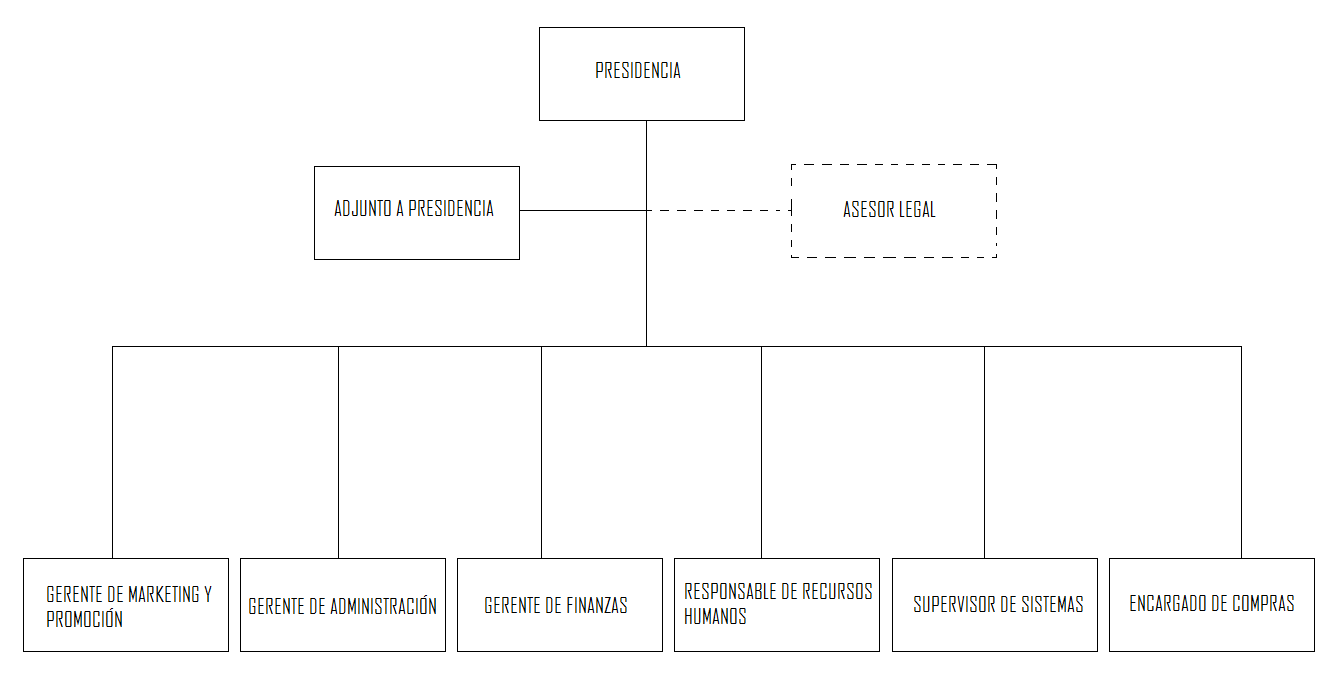
\includegraphics[scale=0.32]{Imagenes/organigrama.png} 
		\end{figure}		
	
	
	\end{frame}
	
	\section{Problemas identificados}
		\begin{frame}%[allowframebreaks]
		\frametitle{Dise�o y Cambio Organizacional}		
			\begin{itemize}
				\item Falta de conduccion y estrategia.
				\item Estrato dirigencial sobredimensionado.
				\item Falta de comunicacion y colaboracion entre las areas.
				\item Falta de reestructuracion luego de los recortes de personal.
				\item Poca confianza en la Direccion General.

			\end{itemize}
		\end{frame}	
	
		\begin{frame}%[allowframebreaks]
		\frametitle{Ingenieria del Producto}		
			\begin{itemize}
				\item Falta de agregado del valor.
				\item No se utilizan los resultados de Investigaciones de Marketing.

				\item Malas inversiones comerciales.

			\end{itemize}
		\end{frame}	
	
		\begin{frame}%[allowframebreaks]
		\frametitle{Marketing}		
			\begin{itemize}
				\item Imagen Comercial
			
			\end{itemize}
		\end{frame}	
	
		\begin{frame}%[allowframebreaks]
		\frametitle{Inestabilidad Financiera}		
			\begin{itemize}
				\item Atraso en el pago de sueldos.
				\item Despidos masivos para reducir costos.
			\end{itemize}
		
		\begin{figure}[H]
		\centering
		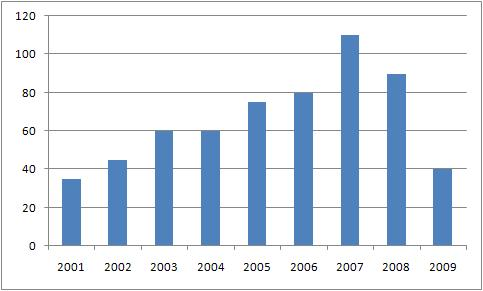
\includegraphics[scale=0.50]{Imagenes/EmpleadosEfect.jpg} 
		\caption{Empleados Efectivos}
		\end{figure}		
		
		\end{frame}	
	
	\section{Solucion Propuesta}
		\begin{frame}%[allowframebreaks]
		\frametitle{Estrategia Propuesta}		
			\begin{itemize}
				\item Reducir la estructura de la empresa.

				\item Centrar a la empresa en pocos productos.

				\item Motivar al personal.
				\item Redistribuir la fuerza de trabajo entre las distintas �reas.
				\item Evitar la p�rdida de personal con inducci�n y la contrataci�n de personal poco capacitado y/o sin experiencia.
			\end{itemize}
		\end{frame}	
		
		
		\subsection*{Reestructuracion de la Organizacion}
		
			\begin{frame}%[allowframebreaks]		
			\frametitle{Organigrama de la Empresa}
				\begin{figure}[H]
				\centering
				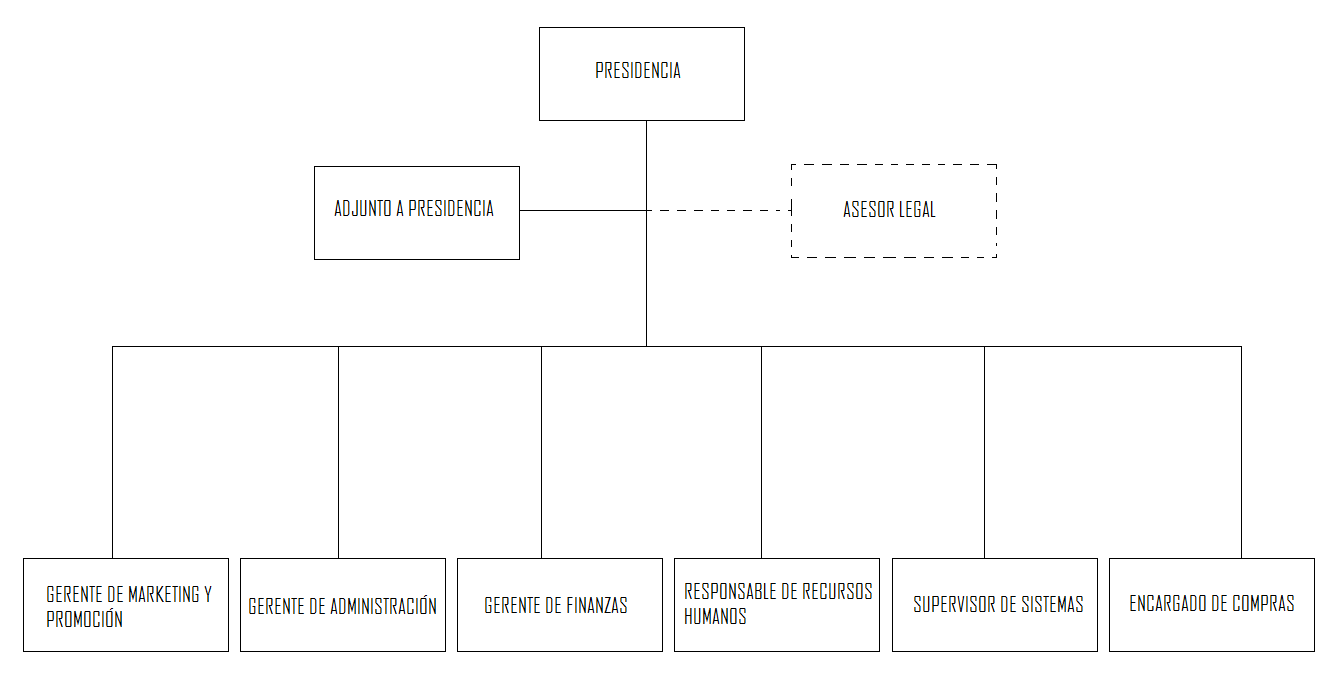
\includegraphics[scale=0.32]{Imagenes/organigrama.png} 
				\end{figure}		
			\end{frame}
			
			\begin{frame}%[allowframebreaks]		
			\frametitle{Problemas estructurales}
			
				\begin{itemize}
					\item Existen departamentos que no figuran en el organigrama.
					\item Gerencias con poca cantidad de empleados, lo cual hace innecesario que sean supervisados por un gerente.
					\item A pesar de la reducci�n de personal,  la empresa sigue manteniendo la misma estructura.

				\end{itemize}

			\end{frame}
			
			\begin{frame}%[allowframebreaks]		
			\frametitle{Cambios estructurales propuestos}
			
				\begin{itemize}
					\item Fusi�n del Departamento de Finanzas con el de Administraci�n.  Subordinaci�n a �el del encargado de RRHH.

					\item Integraci�n del �rea de Compras dentro de la Gerencia de Producto.  Formalizaci�n del �rea de Planificaci�n.

					\item Coordinaci�n del �rea de Marketing y Ventas dentro de la Gerencia de Comercializaci�n.

					\item Armado de comit� entre integrantes de las distintas gerencias.  El Asesor Legal esta vinculado con el comit�,  perdiendo comunicaci�n directa con la presidencia. 					
				\end{itemize}

			\end{frame}

			\begin{frame}%[allowframebreaks]		
			\frametitle{Organigrama de la Empresa}
				\begin{figure}[H]
				\centering
				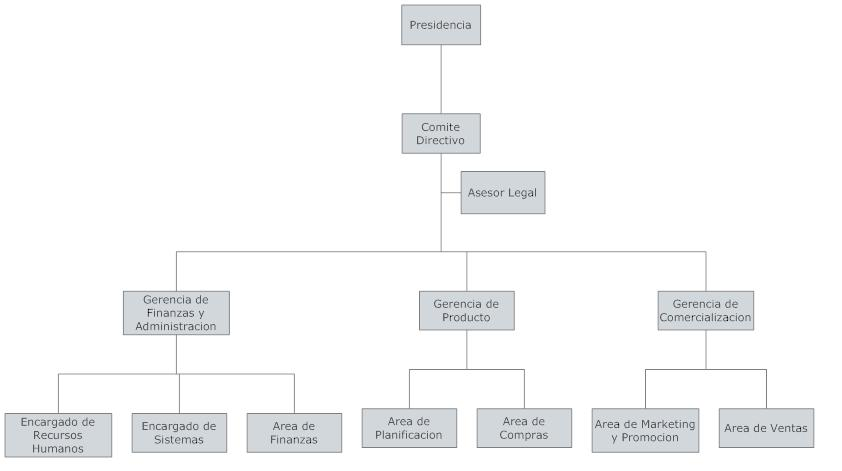
\includegraphics[scale=0.40]{Imagenes/organigramaNuevo.jpg} 
				\end{figure}		
			\end{frame}
	
		\subsection*{Cambios no estructurales}
			\begin{frame}%[allowframebreaks]		
			\frametitle{Cambios no estructurales}
			
				\begin{itemize}
					\item Cambio de imagen de la empresa.
					
					\item Evitar recambios de personal.

					\item Mejora de la Ingenieria de Producto. 

				\end{itemize}

			\end{frame}
	
	
\end{document}